\chapter{人脸检测算法}
\label{chap:facedetection}

人脸检测算法自上世纪以来已经被无数研究者探究过,检测的准确率也是逐年提高。在本系统中,我们需要的是一个能够优秀的处理大角度人脸、模糊人脸甚至部分被遮挡人脸的检测算法。在保证非常高的准确率的同时,该算法需要有非常快的执行速度,以适应同时处理大量图片的需求。

CFDDB测试集中全部的人脸数量为$face_{all}$,检测正确的人脸数量为$face_{right}$,定义检测率$r$为:

\begin{displaymath}
\label{eq:rdef}
	r = \frac{face_{right}}{face_{all}} 
\end{displaymath}

以CFDDB中的图片为标准,我们要求人脸检测算法需要在 定义的$r\geq 80\%$的情况下,在一张Nvidia 1080 Ti显卡的支持下处理一张宽1600像素,高1200像素的图片的平均速度不超过\SI{250}{ms}。


\section{基于HAAR特征的级联分类器}

\subsection{概述}
HAAR特征在物体检测领域有着广泛的应用,在2001年,Paul Viola和Michael Jones在论文[9]中提出了使用HAAR特征来检测人脸的方法。这种方法的基本思想是在一系列含有人脸区域的正图像和不含人脸的负图像上训练训练一系列的分类器,然后将分类器级联组合,得到完成的人脸检测函数。在分类器的训练中,我们通过提取提取图\ref{fig:HAAR}所示的三种不同种类HAAR特征来判断一个特定的区域是否属于人脸区域。

\begin{figure}[!htp]
	\centering
	\subcaptionbox{边特征\label{fig:HAAR:A}}
	{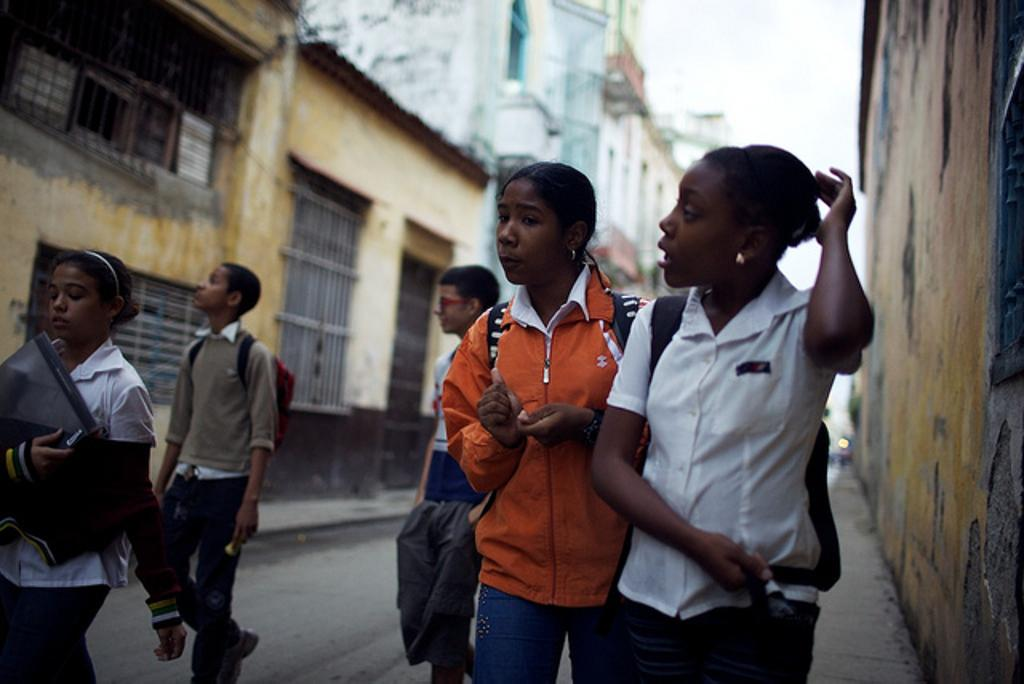
\includegraphics[height=3cm]{chap2/1.jpg}}
	\hspace{4em}
	\subcaptionbox{四矩形特征\label{fig:HAAR:B}}
	{
\includegraphics[height=3cm]{chap2/2.jpg}}
	\hspace{4em}
	\subcaptionbox{线特征\label{fig:HAAR:C}}
	{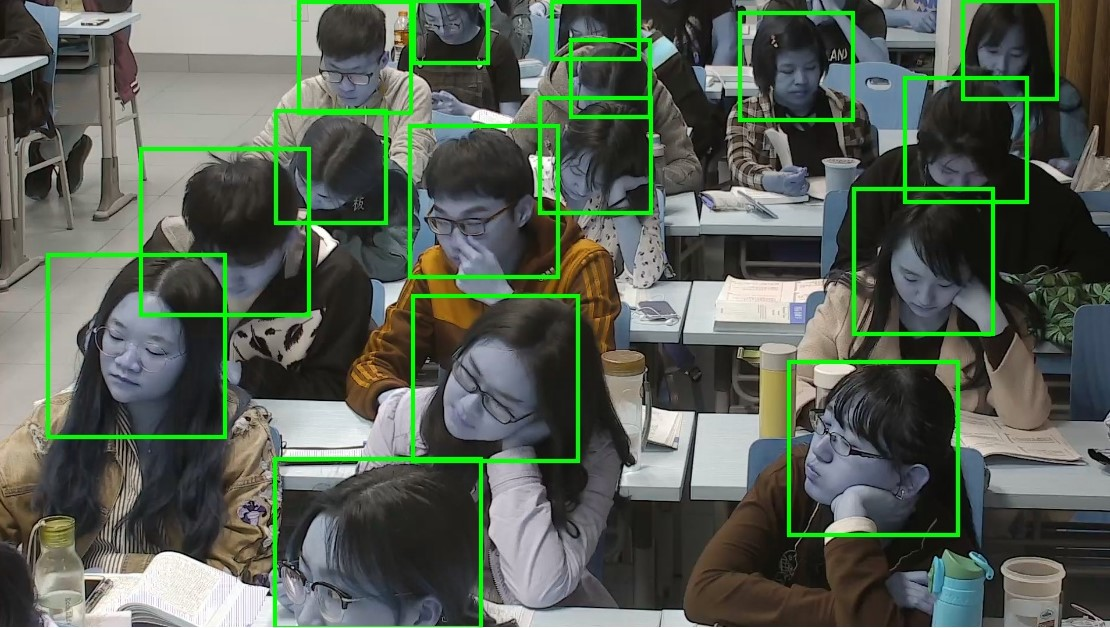
\includegraphics[height=3cm]{chap2/3.jpg}}
	\bicaption{三种HAAR特征}{Three HAAR features}
	\label{fig:HAAR}
\end{figure}

在提取特征前,需要将图像转化为灰度图。三种特征中,图\ref{fig:HAAR:A}的边特征和图\ref{fig:HAAR:C}的线特征在顺时针旋转90度之后提取的特征归为同类特征。特征值的是将某一个特征中黑色部分区域的灰度值之和减去白色区域灰度值之和得到的。

同一种类的特征区域的大小可以不同,提取特征的图片区域可以不同,这样就导致了即使是非常小的一张图片,其所能够提取到的HAAR特征也是非常多的。例如,在一张宽24像素,高24像素的图片中,可以提取的特征可以超过了16万种。如果选取所有的特征进行比对,那么所花费的计算代价是不可接受的。因此,必须对特征进行选择。

首先,对每个特征进行训练,让它可以在训练集上尽可能区分开有人脸的图片和没有人脸的图片。接着计算这个特征的错误率。在所有特征都训练完毕之后选取错误率最小的部分特征作为需要的特征保留。最后,将选取的特征加权求和,作为一个分类器使用。

根据论文[9]中的叙述,每一个特征单独的分类效果较差,但是将所有特征加权求和得到的分类器则非常强大。使用200特征则可达到$95\%$以上的准确率。论文中最终的分类器使用了约6000个特征,具有非常强大的检测能力。

然而,对于一张图片所有可能的区域计算6000个特征仍然是一件非常耗时的工作,对此,作者提出了使用级联分类器的方法来解决。所谓级联,就是将分类器串接起来,只有通过前面分类器检测的图片区域才会继续进行下一分类器的检测。在文章中,分类器共有38级,平均每个区域的识别所需要提取约10个特征。这样的方式极大的加快了分类器的处理速度。

\subsection{在CFDDB上的测试结果}

我们使用OpenCV预训练好的HAAR级联分类器[10]进行检测。这个分类器共有两个可变参数,minNeighbor和scaleFactor。其中minNeighbor表示构成人脸区域的相邻的小矩形个数,scaleFactor表示在两次相继的扫描中,搜索框的比例系数。为了更好的检测HAAR级联分类器的效果,我们选取了不同的minNeighbor和scaleFactor参数在CFDDB上进行了测试,表\ref{tab:haar}为测试结果:

\begin{table}[!hpb]
	\centering
	\bicaption[HAAR级联分类器在CFDDB上的测试结果]
	{HAAR级联分类器在CFDDB上的测试结果}
	{HAAR cascade classifier results on CFDDB}
	\label{tab:haar}
	\begin{tabular}{ ccccc | c }
		\hline
		minNeighbor & scaleFactor & faceDetected & faceRight & totalTime & r\\
		\hline
		2 & 1.1 & 624 & 534 & 27.21s & $49.13\%$\\
		3 & 1.1 & 451 & 394 & 28.62s & $36.25\%$\\
		4 & 1.1 & 379 & 334 & 26.70s & $30.73\%$\\
		5 & 1.1 & 331 & 297 & 26.32s & $27.32\%$\\
		6 & 1.1 & 302 & 272 & 26.37s & $25.02\%$\\
		\hline
		2 & 1.2 & 383 & 333 & 17.03s & $30.63\%$\\
		3 & 1.2 & 294 & 259 & 17.06s & $23.83\%$\\
		4 & 1.2 & 237 & 213 & 16.70s & $19.60\%$\\
		5 & 1.2 & 207 & 187 & 16.73s & $17.20\%$\\
		6 & 1.2 & 181 & 167 & 17.50s & $15.36\%$\\
		\hline
		2 & 1.3 & 295 & 261 & 13.02s & $24.01\%$\\
		3 & 1.3 & 222 & 201 & 13.24s & $18.49\%$\\
		4 & 1.3 & 186 & 172 & 12.90s & $15.82\%$\\
		5 & 1.3 & 161 & 148 & 13.07s & $13.62\%$\\
		6 & 1.3 & 144 & 132 & 13.19s & $12.14\%$\\
		\hline
	\end{tabular}
\end{table}

\subsection{结果分析}

\subsubsection{处理速度}

从图\ref{fig:haartest:speed}中可以清楚的看出,scaleFactor是影响处理速度的主要因素,scaleFactor越大,处理速度越快。而minNeighbor参数则几乎不影响处理速度。HAAR级联分类器在识别率最高时,处理CFDDB中的一张图片的平均速度没有超过250ms,符合本系统的需求。

\begin{figure}[!htp]
	\centering
	\subcaptionbox{边特征\label{fig:haartest:speed1}}
	{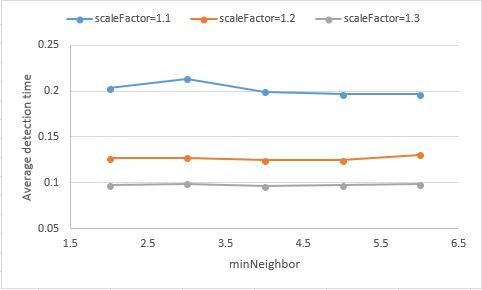
\includegraphics[height=3cm]{chap2/4.jpg}}
	\hspace{4em}
	\subcaptionbox{四矩形特征\label{fig:haartest:speed2}}
	{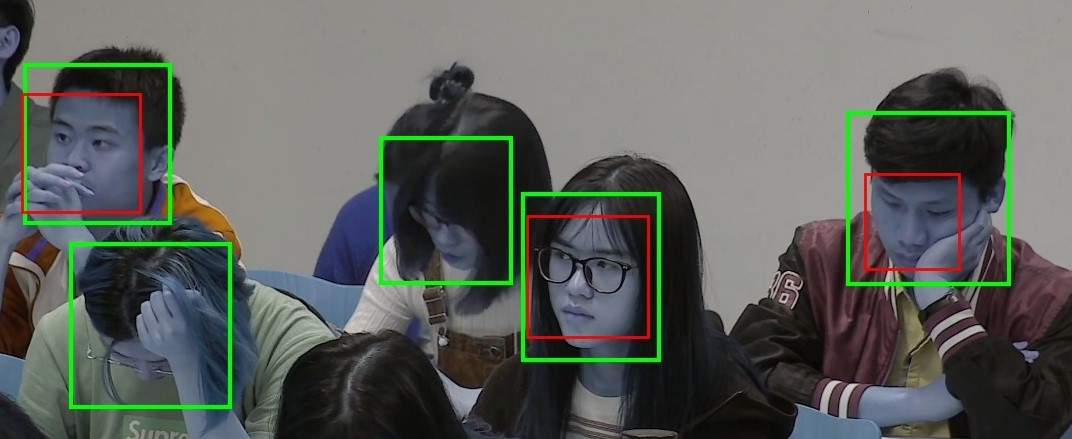
\includegraphics[height=3cm]{chap2/5.jpg}}
	\hspace{4em}
	\label{fig:haartest:speed}
\end{figure}

HAAR级联分类器在CFDDB上检测率最高尚未超过$50\%$,没有达到本系统的需求

\section{HOG}

\subsection{概述}

\subsection{在CFDDB上的测试结果}


\section{SSH}

\subsection{概述}

\subsection{在CFDDB上的测试结果}

